\documentclass[12pt]{article}

%% Language and font encodings
\usepackage[utf8]{inputenc}
\usepackage[english, russian]{babel}
\usepackage[T1,T2A]{fontenc}
%\usepackage[backend=biber,style=alphabetic]{biblatex}   

%% Sets page size and margins
\usepackage[a4paper,top=3cm,bottom=2cm,left=3cm,right=3cm,marginparwidth=1.75cm]{geometry}

\usepackage[backend=biber,style=numeric,sorting=none]{biblatex}
\bibstyle{biblatex}
\bibdata{references,bib}
\citation{biblatex-control}
\bibliography{references}

\usepackage{amsfonts}
\usepackage{amsmath}
\usepackage{indentfirst}
\usepackage{graphicx}
\usepackage{color}
\usepackage[colorlinks=true, allcolors=black]{hyperref}
\usepackage{multirow}

%% Text formatting
\usepackage{indentfirst}
\usepackage{setspace}
\usepackage{mdwlist}
\usepackage{float}
\usepackage{url}

\frenchspacing
\sloppy

\newcommand{\ENGLISH}[1]{#1}
\newtheorem{defn}{Определение}


\title{\bf{Рекуррентные нейронные сети с механизмом внимания для анализа тональности русских текстов}}
\author{Иванов Илья Сергеевич\\студент\\ФИВТ МФТИ}
\date{}
\begin{document}
\maketitle

\section{Введение}
С появлением в Интернете социальных медиа ресурсов, таких как социальные сети, форумы, блоги и др. наблюдается рост как количества пользователей этих ресурсов, так и объема данных, создаваемых пользователями. Люди активно делятся своим мнением в комментариях, обзорах, отзывах, обсуждениях. Эта активность представляет огромный практический интерес со стороны бизнеса, поскольку влияет на покупательскую способность \cite{wang}. В частности, одной из актуальных и практически важных задач для бизнеса является анализ тональности \cite{mokoron2012}. Интерес к данной области стал активно проявляться в последние годы. Существует несколько ежегодных соревнований, такие как, например, соревнование по созданию систем автоматического анализа тональности на английском языке SemEval \cite{semeval2010}, которое проходит с 2010 года.

Для тестирования алгоритмов определения тональности существует также несколько открытых наборов данных. Для английского языка, например, это обзоры фильмов~\footnote{http://nlp.stanford.edu/sentiment/treebank.html}~\cite{imdb, socher-rdm} и товаров~\footnote{http://jmcauley.ucsd.edu/data/amazon/}~\cite{amazon}. Наилучшие алгоритмы в данной области, основаны на рекурсивных тензорных нейронных сетях~\cite{socher-rdm}.

Для русского языка в рамках соревнований Семинара РОМИП в 2011 году~\cite{romip} был сформирован корпус текстов, содержащий отзывы о книгах, фильмах и товарах. В 2014 году Рубцова Ю.В. создала корпус коротких сообщений Twitter~\cite{mokoron2015}.
На соревновательной дорожке по анализу тональности Dialogue Evaluate 2016~\cite{senti-ru-eval} был представлен корпус сообщений Twitter, посвященный банкам и телекоммуникационным компаниям. Победителем последнего соревнования в 2016 году стало решение, основанное на рекуррентной нейронной сети~\cite{arhipenko}.

В данной работе рассматривается задача классификации русских текстов по тональности. В качестве классификаторов используются такие модели как двунаправленная рекуррентная нейронная сеть~\cite{schuster} и двунаправленная рекуррентная нейронная сеть с механизмом внимания~\cite{bahdanau}. Целью является сравнение данных моделей. Ранее для анализа тональности русского текста не применялись модели с механизмом внимания, хотя они успели показать впечатляющие результаты в задачах классификации англоязычных текстов~\cite{yang-att-2016}. Представленные в работе классификаторы экспериментально проверяются на указанном выше наборе русских сообщений из Twitter, представленных на Dialogue Evaluate 2016.

\section{Задача}
Дана обучающая выборка из русскоязычных сообщений с метками трёх классов: -1 (негативная тональность), 0 (нейтральное сообщение), 1 (позитивная тональность). Используя данную выборку, требуется построить классификатор, наиболее точно распознающий тональность сообщений. Целевой метрикой является макро-усреднённая F1-мера по классам позитивной и негативной тональностей.

\section{Алгоритм}
Предварительно текст обрабатывается при помощи Python библиотеки \ENGLISH{\texttt{pymorphy2}}, позволяющей проводить лемматизацию слов. Для получения векторных представлений слов используется алгоритм Word2Vec. Далее последовательность векторов, кодирующая одно сообщение, подается на вход рекуррентной сети.

\subsection{Рекуррентная нейронная сеть}
Ключевой компонентой алгоритма решения поставленной задачи является однослойная двунаправленная рекуррентная нейронная сеть~\cite{schuster} типа GRU~\cite{cho}. GRU (Gated Recurrent Unit) может быть описан следующими уравнениями:
	\begin{align}
	z_{t}&=\sigma_{g}(W_{z}x_{t}+U_{z}h_{t-1})\\
	r_{t}&=\sigma_{g}(W_{r}x_{t}+U_{r}h_{t-1})\\
	\tilde{h}_{t}&=\tanh(Wx_{t}+U(r_{t}\circ h_{t-1}))\\
	h_{t}&=(1-z_{t})\circ \tilde{h}_{t}+z_{t}\circ h_{t-1}
	\end{align}	
где $x_{t}$ -- t-ый элемент последовательности, а $h_{t}$ -- внутреннее состояние сети в t-ый момент времени (после обработки $x_{t}$).

Входная последовательность подается на вход одной рекуррентной сети прямым порядком и другой сети - обратным. После чего выходы этих двух слоёв конкатенируются, образуя выходную последовательность $y_{t} = \left[\overrightarrow{h_{t}},\overleftarrow{h_{t}}\right]$. Таким образом строится двунаправленная рекуррентная сеть, архитектура которой изображена на Рис.~\ref{fig:birnn}.

\begin{figure}[h]
  \centering
  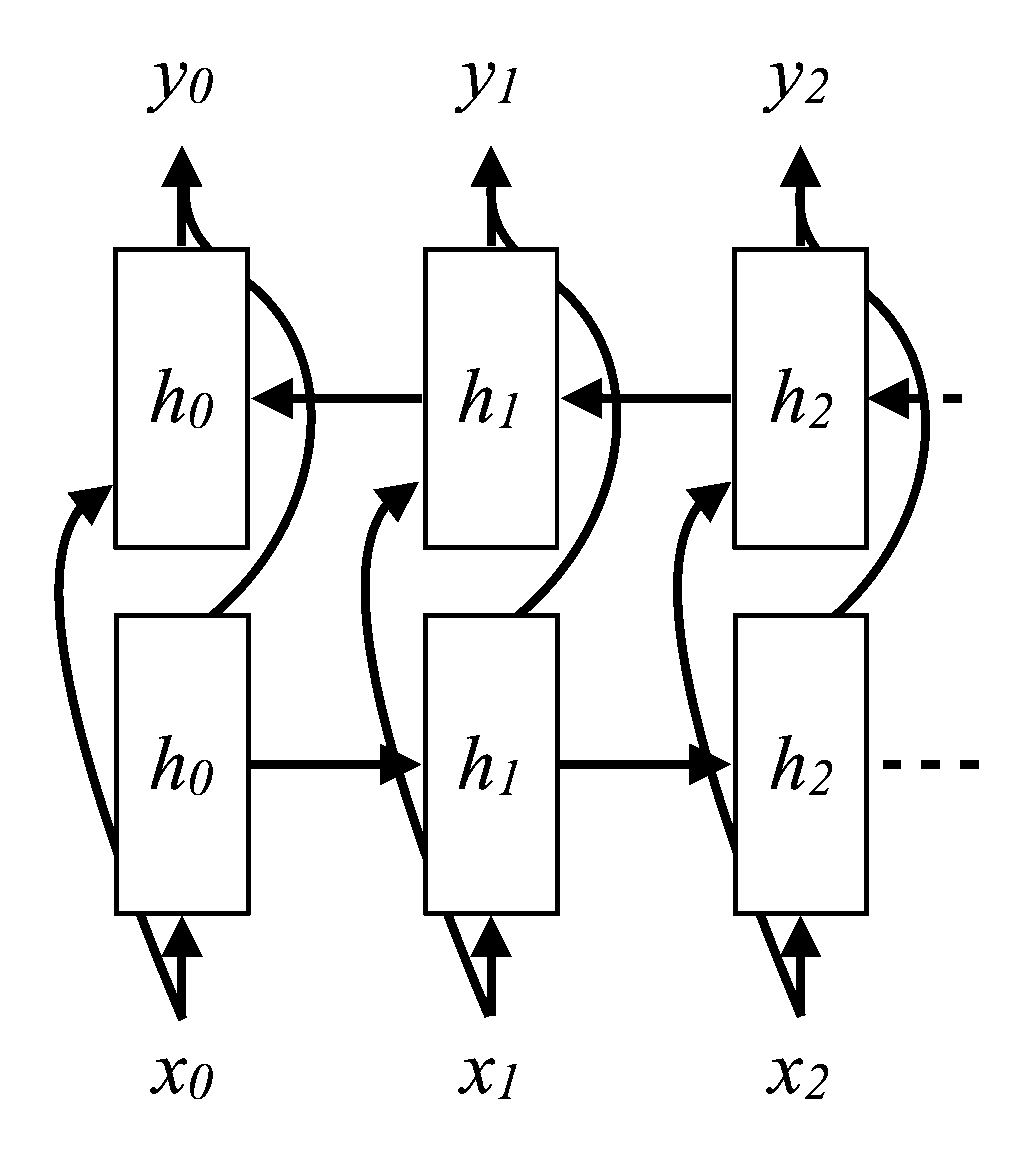
\includegraphics[width=0.4\textwidth]{images/birnn2_bin.png}
  \caption{Двунаправленная рекуррентная нейронная сеть.}
  \label{fig:birnn}
\end{figure}

\subsection{Механизм внимания}
Классическим подходом к работе с выходом нейронной сети является рассмотрение лишь последнего вектора $y_{T}$, где $T$ -- длина входной (и выходной) последовательности, т.к. он аккумулирует в себе извлеченную информацию из всей входной последовательности. Рассматриваемый же нами подход -- механизм внимания~\cite{bahdanau} -- утилизирует все выходные векторы $y_{t}$, вычисляя их линейную комбинацию с коэффициентами $\alpha_{t}$, которые обучаются вместе с остальной сетью. Уравнения механизма внимания выглядят следующим образом:
	\begin{align}	
    \upsilon_{t}&=\tanh{(W_{\omega}y_{t}+b_{\omega})}\\
	\alpha_{t}&=\frac{\exp{(\upsilon_{t}^{T}u_{\omega})}}{\sum_{j=1}^{T}\exp{(\upsilon_{j}^{T}u_{\omega})}}\\
	\upsilon&=\sum_{t=1}^{T}\alpha_{t}y_{t}
	\end{align}	
Архитектура двунаправленной рекуррентной нейронной сети с механизмом внимания представлена на Рис.~\ref{fig:att}. Во время обучения к выходу слоя механизма внимания $\upsilon$ применяется регуляризатор \ENGLISH{Dropout}~\cite{srivastava} для уменьшения переобучения.

\begin{figure}[h]
  \centering
  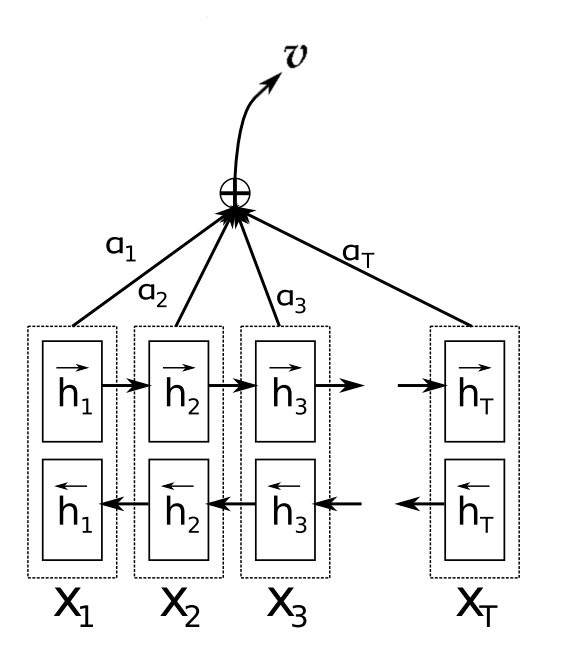
\includegraphics[width=0.5\textwidth]{images/att_edited.png}
  \caption{Двунаправленная рекуррентная нейронная сеть с механизмом внимания.}
  \label{fig:att}
\end{figure}

\subsection{Полносвязанный слой}
После слоя механизма внимания следует полносвязный слой с функцией активации \ENGLISH{softmax}, переводящий вектор $\upsilon$ в трёхмерное пространство, где каждое из чисел обозначает вероятность принадлежности объекта к соответствующему классу:
	\begin{align}	
    \hat{s}&=(\hat{s}^{(-1)},\hat{s}^{(0)},\hat{s}^{(1)})=softmax(W\upsilon+b)
	\end{align}

\section{Обучение}
Классификатор обучается при помощи алгоритма оптимизации Adam, минимизирующего перекрёстную энтропию между выходным распределением $\hat{s}$ и истинным $s$:
    \begin{align}
    L(W)=-\sum_{i=1}^{n}\sum_{c\in\left \{ -1,0,1 \right \}}s_{i}^{(c)}\log{\hat{s_{i}}^{(c)}},
    \end{align}
Параметры модели подбираются при помощи перекрёстной валидации.

\section{Данные}
Организаторами соревнования Dialogue Evaluate 2016 было предложено 2 набора данных. Один содержал сообщения, упоминающие банковские компании, и состоял приблизительно из 12700 экземпляров (9400 в обучающей выборке и 3300 - в тестовой). Второй набор был посвящён телекоммуникационным компания и состоял приблизительно из 10800 экземпляров (8600 в обучающей выборке и 2200 - в тестовой).

\section{Эксперименты}
В Таблице \ref{tab:res} представлены результаты 5-фолд кросс-валидации различных моделей на обучающей выборке и результаты на тестовой выборке. Используемая метрика - макро-усреднённая F1-мера по классам положительной и отрицательной тональностей. Помимо наших экспериментов в таблице представлены результаты победителя~\cite{arhipenko}  и бейзлайны соревновательной дорожки по анализу тональности Dialogue Evaluate 2016~\cite{senti-ru-eval}. Здесь стоит отметить, что решения участников соревнования содержали различные дополнительные методы обработки данных, помимо лемматизации, которые мы не использовали.

Видно, что лишь на одном из двух доменов алгоритм с исследуемым механизмом внимания превзошёл аналогичный алгоритм без механизма внимания. Весь код решения и значения гиперпараметров доступны по ссылке \url{www.github.com/ilivans/tf-rnn-attention}.

\begin{table}[]
\centering
\caption{F1-мера различных моделей на кросс-валидации (CV) и на тестовой выборке}
\label{tab:res}
\begin{tabular}{l|l|l|l|l|}
\cline{2-5}
                                                                                                              & \multicolumn{2}{c|}{Banks}   & \multicolumn{2}{c|}{\begin{tabular}[c]{@{}c@{}}Telecommunication\\ companies\end{tabular}} \\ \cline{2-5}                                                                                                               
                                                                                                              & \begin{tabular}[c]{@{}l@{}}5-fold CV\\(mean, std)\end{tabular}  & test & \begin{tabular}[c]{@{}l@{}}5-fold CV\\(mean, std)\end{tabular}                                & test                                \\ \hline
\multicolumn{1}{|l|}{Bi-GRU}                                                                                  & 0.74, 0.02            & 0.48 & 0.62, 0.01                                                     & 0.52                                \\ \hline
\multicolumn{1}{|l|}{Bi-GRU + Attention}                                                                      & 0.74, 0.02            & 0.51 & 0.60, 0.02                                           & 0.49                                \\ \hline
\multicolumn{1}{|l|}{\begin{tabular}[c]{@{}l@{}}2-layer GRU,\\ reversed sequences\\ (Arhipenko)\end{tabular}} & 0.62, -               & 0.55 & 0.66, -                                              & 0.56                                \\ \hline
\multicolumn{1}{|l|}{Bi-GRU (Arhipenko)}                                                                      & 0.62, -               & -    & 0.65, -                                              & -                                   \\ \hline
\multicolumn{1}{|l|}{LSTM (Arhipenko)}                                                                        & 0.60, -               & -    & 0.64, -                                              & -                                   \\ \hline
\multicolumn{1}{|l|}{CNN (Arhipenko)}                                                                         & -                     & 0.48 & -                                                    & 0.47                                \\ \hline
\multicolumn{1}{|l|}{SVM baseline}                                                                            & -                     & 0.46 & -                                                    & 0.46                                \\ \hline
\multicolumn{1}{|l|}{Majority baseline}                                                                       & -                     & 0.31 & -                                                    & 0.19                                \\ \hline
\end{tabular}
\end{table}

Также из таблицы видно, что значения F1-меры на обучающей и тестовой выборке существенно отличаются. Мы провели ряд экспериментов, для того чтобы найти гиперпараметры, при которых бы отсутствовало переобучение алгоритмов. Однако эта разница наблюдалась во всех наших экспериментах, как при уменьшении размера сети, так и с увеличением параметра регуляризации dropout~\cite{srivastava}. Чтобы исследовать причины этого расхождения, мы провели эксперимент со смешиванием обучающей и тестовой выборок и последующей кросс-валидацией моделей на смешанной выборке. Результаты данного эксперимента приведены в Таблице \ref{tab:mix}. Стоит отметить, что размеры обучающей и тестовой выборок сравнимы (5:2). Судя по тому, что кросс-валидация на смешанной выборке показала результаты очень близкие к кросс-валидации на обучающей выборке, можно предположить, что между обучающей и тестовой выборками есть существенные различия. Однако для тщательной проверки этой гипотезы требуется провести детальный сравнительный анализ данных, что авторы планируют проделать в будущем.

\begin{table}[]
\centering
\caption{Результаты эксперимента со смешиванием обучающей и тестовой выборок}
\label{tab:mix}
\begin{tabular}{l|c|l|l|c|l|l|}
\cline{2-7}
                                         & \multicolumn{3}{c|}{Banks}                                                                                     & \multicolumn{3}{c|}{\begin{tabular}[c]{@{}c@{}}Telecommunication\\ companies\end{tabular}}                     \\ \cline{2-7} 
                                         & \multicolumn{2}{c|}{cross-validation}                             & \multicolumn{1}{c|}{\multirow{2}{*}{test}} & \multicolumn{2}{c|}{cross-validation}                             & \multicolumn{1}{c|}{\multirow{2}{*}{test}} \\ \cline{2-3} \cline{5-6}
                                         & train                           & \multicolumn{1}{c|}{train+test} & \multicolumn{1}{c|}{}                      & train                           & \multicolumn{1}{c|}{train+test} & \multicolumn{1}{c|}{}                      \\ \hline
\multicolumn{1}{|l|}{Bi-GRU}             & \multicolumn{1}{l|}{0.74, 0.02} & 0.71, 0.02                      & 0.48                                       & \multicolumn{1}{l|}{0.62, 0.01} & 0.62, 0.01                      & 0.52                                       \\ \hline
\multicolumn{1}{|l|}{Bi-GRU + Attention} & \multicolumn{1}{l|}{0.74, 0.02} & 0.72, 0.01                      & 0.51                                       & \multicolumn{1}{l|}{0.60, 0.02} & 0.62, 0.01                      & 0.49                                       \\ \hline
\end{tabular}
\end{table}

Таким образом, исследована применимость модели на основе двунаправленной рекуррентной нейронной сети с механизмом внимания в задаче классификации тональности русскоязычных текстов. Проведено сравнение данной модели с её ранее изученными аналогами. В будущем планируется провести эксперименты на других, более сбалансированных и крупных, наборах данных.

\printbibliography

\end{document}
